\documentclass{beamer}
\usepackage[utf8]{inputenc}

\usetheme{Madrid}
\usecolortheme{default}
\usepackage{amsmath,amssymb,amsfonts,amsthm}
\usepackage{txfonts}
\usepackage{tkz-euclide}
\usepackage{listings}
\usepackage{adjustbox}
\usepackage{array}
\usepackage{tabularx}
\usepackage{gvv}
\usepackage{lmodern}
\usepackage{circuitikz}
\usepackage{tikz}
\usepackage{graphicx}
\usepackage{mathtools}
\setbeamertemplate{page number in head/foot}[totalframenumber]

\usepackage{tcolorbox}
\tcbuselibrary{minted,breakable,xparse,skins}



\definecolor{bg}{gray}{0.95}
\DeclareTCBListing{mintedbox}{O{}m!O{}}{%
  breakable=true,
  listing engine=minted,
  listing only,
  minted language=#2,
  minted style=default,
  minted options={%
    linenos,
    gobble=0,
    breaklines=true,
    breakafter=,,
    fontsize=\small,
    numbersep=8pt,
    #1},
  boxsep=0pt,
  left skip=0pt,
  right skip=0pt,
  left=25pt,
  right=0pt,
  top=3pt,
  bottom=3pt,
  arc=5pt,
  leftrule=0pt,
  rightrule=0pt,
  bottomrule=2pt,
  toprule=2pt,
  colback=bg,
  colframe=orange!70,
  enhanced,
  overlay={%
    \begin{tcbclipinterior}
    \fill[orange!20!white] (frame.south west) rectangle ([xshift=20pt]frame.north west);
    \end{tcbclipinterior}},
  #3,
}
\lstset{
    language=C,
    basicstyle=\ttfamily\small,
    keywordstyle=\color{blue},
    stringstyle=\color{orange},
    commentstyle=\color{green!60!black},
    numbers=left,
    numberstyle=\tiny\color{gray},
    breaklines=true,
    showstringspaces=false,
}
%This block of code defines the information to appear in the
%Title page
\title %optional
{4.11.36}
%\subtitle{A short story}

\author % (optional)
{Vaishnavi - EE25BTECH11059}



\begin{document}


\frame{\titlepage}
\begin{frame}{Question}
Find the coordinates of the point where the line through the points $(3, -4, -5)$ and $(2, -3, 1)$ crosses the plane determined by the points $(1, 2, 3)$, $(4, 2, -3)$ and $(0, 4, 3)$.
\end{frame}
\begin{frame}{allowframebreaks}
\frametitle{Solution}
\begin{table}[H]    
  \centering
  \begin{tabular}{|c|c|}
\hline
\textbf{Name} & \textbf{Value} \\ \hline
$\vec{A}$ & $\myvec{2 & 1 \\0 & 3}$ \\ \hline
\end{tabular}

  \caption{Variables Used}
  \label{tab:1.10.2}
\end{table}

\end{frame}


\begin{frame}{Solution}
Let eq of plane be
\begin{align}
    \vec{n^T}\vec{x}=1
\end{align}
As $\vec{P},\vec{Q},\vec{R}$ lie on the plane
\begin{align}
 \vec{n^T}\vec{P}=1\\
  \vec{n^T}\vec{Q}=1\\
  \vec{n^T}\vec{R}=1\\
   \myvec{P^T 
        \\
        Q^T
        \\
        R^T}
\vec{n}
=
\myvec{1
       \\
       1
       \\
       1}
 \end{align}
\end{frame}

\begin{frame}{solution}
From eq $(2),(3),(4)and (5)$
\begin{align}
\begin{pmatrix}
\begin{array}{ccc|c}
1 & 2 & 3 & 1\\
4 & 2 & -3 & 1\\
0 & 4 & 3 & 1
\end{array}
\end{pmatrix}
&\xrightarrow{R_2 \to R_2 - 4R_1}
\begin{pmatrix}
\begin{array}{ccc|c}
1 & 2 & 3 & 1\\
0 & -6 & -15 & -3\\
0 & 4 & 3 & 1
\end{array}
\end{pmatrix} \\[4pt]
&\xrightarrow{R_2 \to -\tfrac{1}{3}R_2}
\begin{pmatrix}
\begin{array}{ccc|c}
1 & 2 & 3 & 1\\
0 & 2 & 5 & 1\\
0 & 4 & 3 & 1
\end{array}
\end{pmatrix} 
\end{align}
\end{frame}
\begin{frame}{Solutions}
    \begin{align}
&\xrightarrow{R_3 \to R_3 - 2R_2}
\begin{pmatrix}
\begin{array}{ccc|c}
1 & 2 & 3 & 1\\
0 & 2 & 5 & 1\\
0 & 0 & -7 & -1
\end{array}
\end{pmatrix} \\[4pt]
&\xrightarrow{R_3 \to -\tfrac{1}{7}R_3}
\begin{pmatrix}
\begin{array}{ccc|c}
1 & 2 & 3 & 1\\
0 & 2 & 5 & 1\\
0 & 0 & 1 & \tfrac{1}{7}
\end{array}
\end{pmatrix} \\[4pt]
&\xrightarrow{R_2 \to R_2 - 5R_3}
\begin{pmatrix}
\begin{array}{ccc|c}
1 & 2 & 3 & 1\\
0 & 2 & 0 & \tfrac{2}{7}\\
0 & 0 & 1 & \tfrac{1}{7}
\end{array}
\end{pmatrix} 
\end{align}
\end{frame}
\begin{frame}{Solutions}
    \begin{align}
  &\xrightarrow{R_2 \to \tfrac{1}{2}R_2}
\begin{pmatrix}
\begin{array}{ccc|c}
1 & 2 & 3 & 1\\
0 & 1 & 0 & \tfrac{1}{7}\\
0 & 0 & 1 & \tfrac{1}{7}
\end{array}
\end{pmatrix} \\[4pt]
&\xrightarrow{R_1 \to R_1 - 3R_3}
\begin{pmatrix}
\begin{array}{ccc|c}
1 & 2 & 0 & \tfrac{4}{7}\\
0 & 1 & 0 & \tfrac{1}{7}\\
0 & 0 & 1 & \tfrac{1}{7}
\end{array}
\end{pmatrix} \\[4pt]
&\xrightarrow{R_1 \to R_1 - 2R_2}
\begin{pmatrix}
\begin{array}{ccc|c}
1 & 0 & 0 & \tfrac{2}{7}\\
0 & 1 & 0 & \tfrac{1}{7}\\
0 & 0 & 1 & \tfrac{1}{7}
\end{array}
\end{pmatrix}  
\end{align}
\end{frame}
\begin{frame}{Solution}
    \begin{align}
\vec{n}=
\myvec{\frac{2}{7}
       \\
       \frac{1}{7}
       \\
       \frac{1}{7}
}
\end{align}  
hence eq of plane is
\begin{align}
 \myvec{\tfrac{2}{7} & \tfrac{1}{7} & \tfrac{1}{7}} 
 \vec{x}
 =1
\end{align}   
\end{frame}
\begin{frame}{Solutions}

    let a point on line $\vec{A}\vec{B}$ be 
\begin{align}
\vec{c}=k\vec{A}+(1-k)\vec{B}\\
\vec{n^T}(k\vec{A}+(1-k)\vec{B})
=1\\
\myvec{\frac{2}{7} & \frac{1}{7} & \frac{1}{7}}
\myvec{2+k
               \\
              -3-k
              \\
              1-6k
              }
 =1
 4+2k-3-k+1-6k=7\\
2-5k=7\\
k=-1
\end{align}
\end{frame}
\begin{frame}{Solution}
   The point $\vec{c}$ is
\begin{align}
    \vec{c}=\myvec{1
                   \\
                   -2
                   \\
                   7
             }
\end{align} 
\end{frame}





\begin{frame}{Graph}
   Refer to Figure

\begin{figure}[H]
\begin{center}
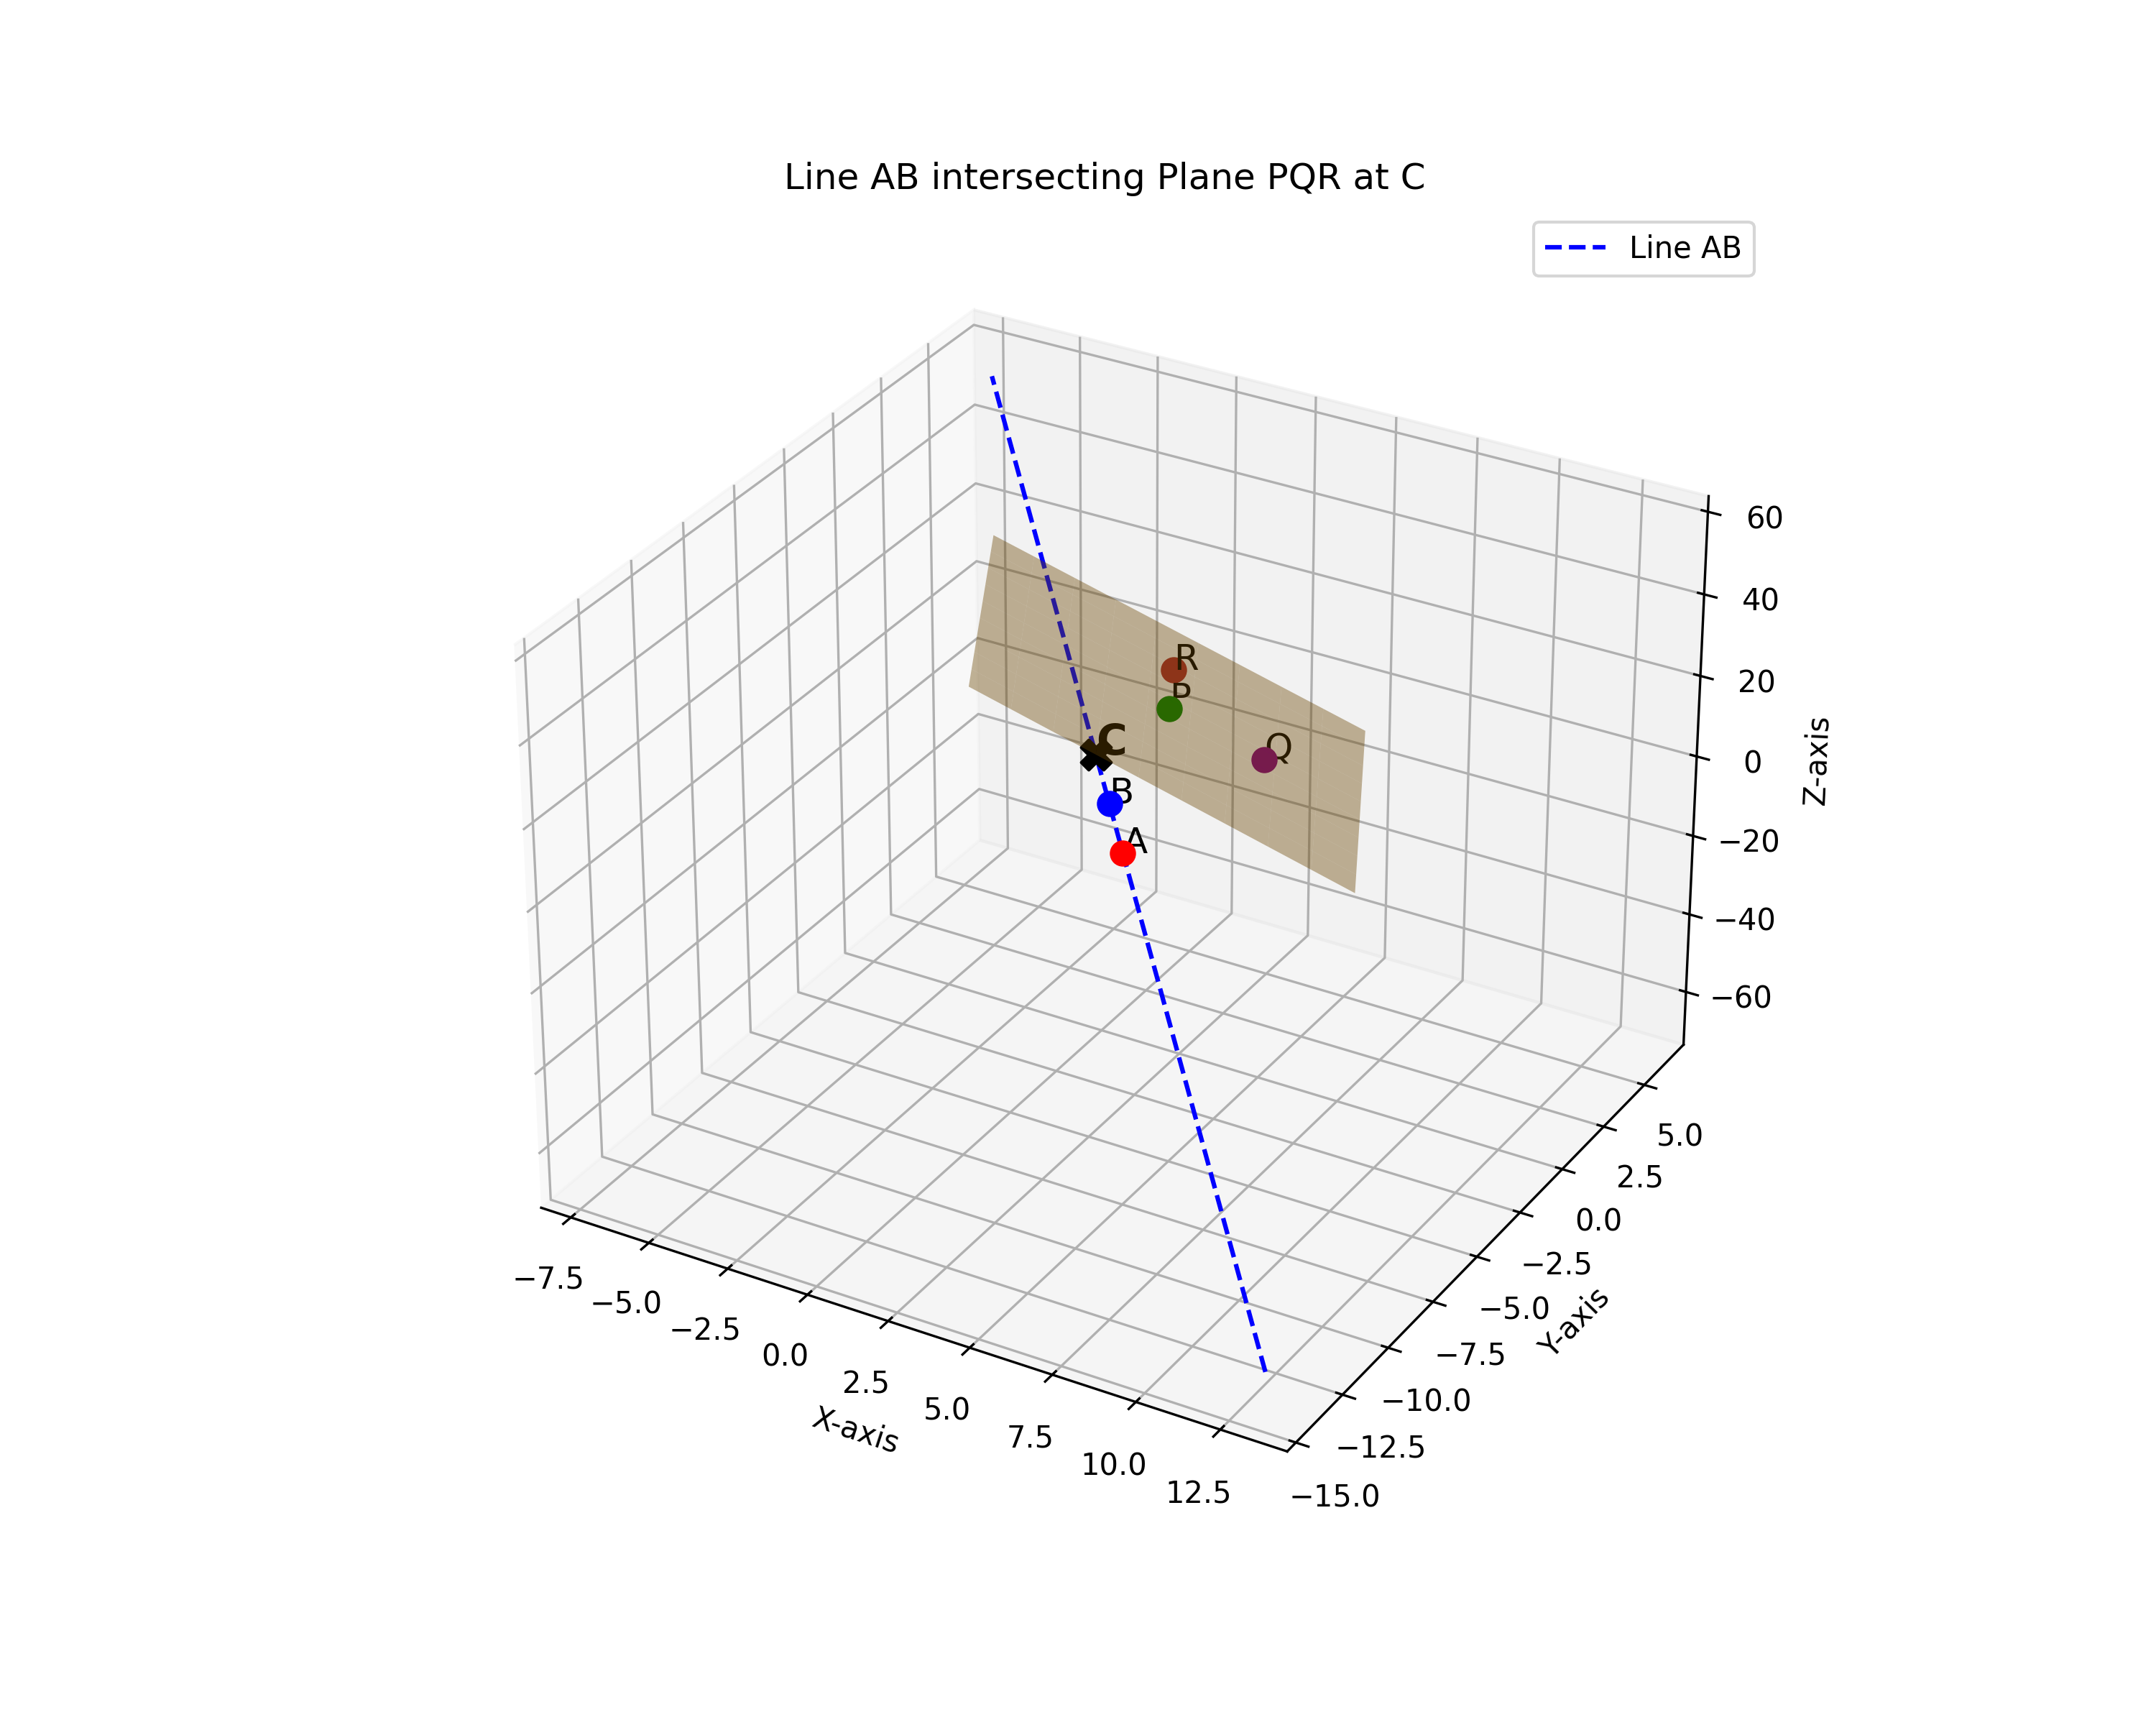
\includegraphics[width=0.6\columnwidth]{../figs/graph8.png}
\end{center}
\caption{}
\label{fig:Fig}
\end{figure}  
\end{frame}




\begin{frame}[fragile]
    \frametitle{Python Code}
    \begin{lstlisting}
import numpy as np
import matplotlib.pyplot as plt
from mpl_toolkits.mplot3d import Axes3D

# Given points
A = np.array([3, -4, -5])
B = np.array([2, -3, 1])
P = np.array([1, 2, 3])
Q = np.array([4, 2, -3])
R = np.array([0, 4, 3])

# Direction vector of line AB
AB = B - A

# Normal vector to plane PQR = (Q-P) x (R-P)
n = np.cross(Q-P, R-P)

# Solve for intersection: A + t*AB lies in plane
t = np.dot(n, P-A) / np.dot(n, AB)
C = A + t*AB  # intersection point

# Generate grid for plane PQR
u = np.linspace(-2, 2, 10)
v = np.linspace(-2, 2, 10)
U, V = np.meshgrid(u, v)
\end{lstlisting}
\end{frame}

\begin{frame}[fragile]
    \frametitle{Python Code }

    \begin{lstlisting}
plane_points = P.reshape(3,1,1) + (Q-P).reshape(3,1,1)*U + (R-P).reshape(3,1,1)*V

# Create plot
fig = plt.figure(figsize=(10, 8))
ax = fig.add_subplot(111, projection='3d')

# Extended line AB
t_vals = np.linspace(-10, 10, 200)
line_points = A.reshape(3,1) + np.outer(AB, t_vals)
ax.plot(line_points[0], line_points[1], line_points[2], 'b--', label="Line AB")

# Plot plane
ax.plot_surface(plane_points[0], plane_points[1], plane_points[2], alpha=0.4, color='orange')

# Plot points
ax.scatter(*A, color='red', s=60)
ax.text(*A, "A", fontsize=12)

ax.scatter(*B, color='blue', s=60)
ax.text(*B, "B", fontsize=12)


    \end{lstlisting}
\end{frame}

\begin{frame}[fragile]
    \frametitle{Python Code}

    \begin{lstlisting}
ax.scatter(*P, color='green', s=60)
ax.text(*P, "P", fontsize=12)

ax.scatter(*Q, color='purple', s=60)
ax.text(*Q, "Q", fontsize=12)

ax.scatter(*R, color='brown', s=60)
ax.text(*R, "R", fontsize=12)

ax.scatter(*C, color='black', s=100, marker='X')
ax.text(*C, "C", fontsize=14, color='black', weight='bold')

# Labels
ax.set_xlabel("X-axis")
ax.set_ylabel("Y-axis")
ax.set_zlabel("Z-axis")
ax.set_title("Line AB intersecting Plane PQR at C")

plt.legend()
plt.savefig("graph8.png", dpi=300)
plt.show()

print("Intersection Point C =", C)



  \end{lstlisting}
\end{frame}

\begin{frame}[fragile]
\frametitle{C Code}
\begin{lstlisting}
#include <stdio.h>
#include <math.h>

#define N 3

// Gaussian elimination solver
void gaussElimination(double A[N][N], double b[N], double x[N]) {
    int i, j, k;
    double ratio;

    // Forward elimination
    for (i = 0; i < N - 1; i++) {
        for (j = i + 1; j < N; j++) {
            if (fabs(A[i][i]) < 1e-12) return;
          
    \end{lstlisting}

\end{frame}
\begin{frame}[fragile]
\frametitle{C Code}
\begin{lstlisting}
  ratio = A[j][i] / A[i][i];
            for (k = 0; k < N; k++) {
                A[j][k] -= ratio * A[i][k];
            }
            b[j] -= ratio * b[i];
        }
    }
    // Back substitution
    for (i = N - 1; i >= 0; i--) {
        x[i] = b[i];
        for (j = i + 1; j < N; j++) {
            x[i] -= A[i][j] * x[j];
        }
        x[i] /= A[i][i];
    }
}
    \end{lstlisting}

\end{frame}

\begin{frame}[fragile]
\frametitle{C Code}
\begin{lstlisting}
 

// Exposed function for Python
void solve_plane(double *out) {
    double A[N][N] = {
        {1, 2, 3},
        {4, 2, -3},
        {0, 4, 3}
    };
    double b[N] = {1, 1, 1};
    double n[N];

    gaussElimination(A, b, n);

    for (int i = 0; i < N; i++) {
        out[i] = n[i];
    }
}

\end{lstlisting}
\end{frame}

\begin{frame}[fragile]
\frametitle{Python and C Code}

\begin{lstlisting}
import ctypes
import numpy as np

# Load shared library
lib = ctypes.CDLL("./code.so")

# Define function signature: void solve_plane(double *out)
lib.solve_plane.argtypes = [ctypes.POINTER(ctypes.c_double)]
lib.solve_plane.restype = None

# Prepare output array
out = (ctypes.c_double * 3)()
lib.solve_plane(out)

# Convert to numpy for convenience
normal_vec = np.array([out[i] for i in range(3)])
print("Normal vector:", normal_vec)


\end{lstlisting}

\end{frame}

\end{document}